\documentclass{beamer}

\usepackage[T1]{fontenc} % Obsługuje polskie znaki
\usepackage[utf8]{inputenc} % Kodowanie UTF-8
\usepackage{amsmath} % Matematyka
\usepackage{lmodern} % Użycie nowoczesnej czcionki
\usepackage{xcolor} % Załaduj pakiet xcolor

% Zdefiniowanie koloru darkblue
\definecolor{darkblue}{rgb}{0.0, 0.0, 0.5}

% Zmiana koloru tła tytułów slajdów
\setbeamercolor{frametitle}{bg=darkblue, fg=white} % Niebieski tytuł i biały tekst

% Kolor tła slajdów
\setbeamercolor{background canvas}{bg=white} % Białe tło

\title{Fisherowska dyskryminacja liniowa – zastosowanie dla nowych danych}
\author{Imię i Nazwisko}
\date{\today}

\begin{document}

% Tytułowy slajd
\begin{frame}
    \titlepage
\end{frame}

% Slajd 1: Wprowadzenie
\begin{frame}
    \frametitle{Wprowadzenie}
    Fisherowska dyskryminacja liniowa (LDA) jest techniką statystyczną wykorzystywaną w analizie danych. Jej celem jest maksymalizacja rozróżnienia między klasami w zbiorze danych. Wykorzystywana jest głównie w klasyfikacji.
    \begin{itemize}
        \item LDA znajduje liniową kombinację cech, która najlepiej oddziela klasy.
        \item Jest szeroko stosowana w wielu dziedzinach, takich jak biologia, rozpoznawanie twarzy czy analiza tekstów.
    \end{itemize}
\end{frame}

% Slajd 2: Historia metody
\begin{frame}
    \frametitle{Historia metody}
    Fisherowska dyskryminacja liniowa została zaproponowana przez Ronalda A. Fishera w 1936 roku. Początkowo była stosowana w analizie danych botanicznych, aby rozróżnić różne gatunki roślin na podstawie pomiarów ich cech morfologicznych.
\end{frame}





\begin{frame}{Motywacja do stosowania LDA}
    Wyobraźmy sobie, że mamy dwie klasy (np. Klasa A i Klasa B), które chcemy skutecznie od siebie oddzielić. Każda klasa może być opisana przez wiele różnych cech, takich jak:
    \begin{itemize}
        \item Wzrost, waga,
        \item Wiek, poziom wykształcenia,
        \item Wyniki testów itp.
    \end{itemize}
    
    \bigskip
    **Problem z jedną cechą:** Jeśli użyjemy tylko jednej cechy (np. wzrostu), klasy mogą częściowo się nakładać. Nie będziemy w stanie jednoznacznie przypisać danych punktów do jednej z klas.

    \bigskip
    \textbf{Przykład:} Przykład danych w przestrzeni 1D, gdzie klasy nachodzą na siebie.
    
    \bigskip
    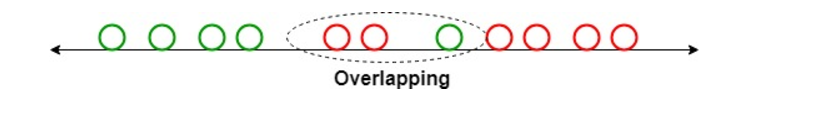
\includegraphics[width=0.7\textwidth]{C:/Users/marci/OneDrive/Pulpit/Opty - prezentacja/overlapping.png} 
\end{frame}














% Slajd 3: Matematyczne podstawy
\begin{frame}
    \frametitle{Matematyczne podstawy}
    Fisherowska dyskryminacja liniowa polega na znalezieniu takiej linii (hiperpłaszczyzny), która maksymalizuje stosunek wariancji między klasami do wariancji wewnątrz klas.
    
    Wzór na funkcję celu:
    \[
    J(\mathbf{w}) = \frac{\mathbf{w}^T S_B \mathbf{w}}{\mathbf{w}^T S_W \mathbf{w}}
    \]

    Gdzie:
    \begin{itemize}
        \item \( S_B \) - macierz rozrzutu między klasami,
        \item \( S_W \) - macierz rozrzutu wewnątrz klas,
        \item \( \mathbf{w} \) - wektor wag, który określa kierunek linii separującej.
    \end{itemize}
\end{frame}



% Nowy slajd: Wyprowadzenie optymalnego \mathbf{w}
\begin{frame}
    \frametitle{Wyprowadzenie optymalnego \(\mathbf{w}\)}
    Celem jest maksymalizacja funkcji celu:
    \[
    J(\mathbf{w}) = \frac{\mathbf{w}^T S_B \mathbf{w}}{\mathbf{w}^T S_W \mathbf{w}}
    \]
    Aby znaleźć optymalny wektor \(\mathbf{w}\), liczymy pochodną \(\nabla J(\mathbf{w})\) względem \(\mathbf{w}\):
    \[
    \nabla J(\mathbf{w}) = 0
    \]
    Rozwijamy krok po kroku w kolejnych slajdach.
\end{frame}

% Slajd: Liczenie pochodnej
\begin{frame}
    \frametitle{Liczenie pochodnej \(\nabla J(\mathbf{w})\)}
    Funkcja celu:
    \[
    J(\mathbf{w}) = \frac{\mathbf{w}^T S_B \mathbf{w}}{\mathbf{w}^T S_W \mathbf{w}}
    \]
    Liczymy pochodną z licznika i mianownika:
    \[
    \nabla \left( \mathbf{w}^T S_B \mathbf{w} \right) = 2 S_B \mathbf{w}, \quad 
    \nabla \left( \mathbf{w}^T S_W \mathbf{w} \right) = 2 S_W \mathbf{w}
    \]
    Stosujemy wzór na pochodną ilorazu:
    \[
    \nabla J(\mathbf{w}) = \frac{2 S_B \mathbf{w} \cdot (\mathbf{w}^T S_W \mathbf{w}) - 2 S_W \mathbf{w} \cdot (\mathbf{w}^T S_B \mathbf{w})}{(\mathbf{w}^T S_W \mathbf{w})^2}
    \]
    Szukamy, kiedy \(\nabla J(\mathbf{w}) = 0\).
\end{frame}



% Slajd: Warunek stacjonarności
\begin{frame}
    \frametitle{Warunek stacjonarności}
    Aby znaleźć maksimum funkcji celu, przyrównujemy pochodną do zera:
    \[
    \nabla J(\mathbf{w}) = 0
    \]
    Co oznacza, że:
    \[
    S_B \mathbf{w} (\mathbf{w}^T S_W \mathbf{w}) = S_W \mathbf{w} (\mathbf{w}^T S_B \mathbf{w})
    \]
    Dzielimy obie strony przez \((\mathbf{w}^T S_W \mathbf{w})\):
    \[
    S_B \mathbf{w} = \frac{\mathbf{w}^T S_B \mathbf{w}}{\mathbf{w}^T S_W \mathbf{w}} S_W \mathbf{w}
    \]
    Definiujemy:
    \[
    \lambda = \frac{\mathbf{w}^T S_B \mathbf{w}}{\mathbf{w}^T S_W \mathbf{w}}
    \]
\end{frame}






% Slajd: Przejście do równania własnego
\begin{frame}
    \frametitle{Przejście do równania własnego}
    Otrzymane równanie:
    \[
    S_B \mathbf{w} = \lambda S_W \mathbf{w}
    \]
    Przemnażamy obustronnie przez \( S_W^{-1} \) (zakładamy, że \( S_W \) jest odwracalna):
    \[
    S_W^{-1} S_B \mathbf{w} = \lambda \mathbf{w}
    \]
    Jest to równanie własne, gdzie:
    \begin{itemize}
        \item \( S_W^{-1} S_B \) - macierz,
        \item \(\lambda\) - wartość własna,
        \item \(\mathbf{w}\) - wektor własny.
    \end{itemize}
\end{frame}







% Slajd: Interpretacja
\begin{frame}
    \frametitle{Interpretacja równania własnego}
    \begin{itemize}
        \item Rozwiązujemy równanie \( S_W^{-1} S_B \mathbf{w} = \lambda \mathbf{w} \).
        \item Wartości własne \(\lambda\) określają zdolność rozróżnienia klas.
        \item Optymalny wektor \(\mathbf{w}\) to ten, który odpowiada największemu \(\lambda\).
    \end{itemize}
    Podsumowanie:
    \[
    \mathbf{w} = \text{wektor własny dla największej } \lambda
    \]
    \[
    J(\mathbf{w}) \text{ maksymalizowane przy } \lambda_{\text{max}}
    \]
\end{frame}






% Slajd: Rozwiązanie równania
\begin{frame}
    \frametitle{Rozwiązanie równania}
    Z równania \(\nabla J(\mathbf{w}) = 0\) wynika, że optymalny \(\mathbf{w}\) musi spełniać:
    \[
    S_W^{-1} S_B \mathbf{w} = \lambda \mathbf{w}
    \]
    Gdzie \(\lambda\) to wartość własna układu. Rozwiązaniem jest:
    \begin{itemize}
        \item \(\mathbf{w}\) - wektor własny macierzy \(S_W^{-1} S_B\),
        \item \(\lambda\) - odpowiadająca wartość własna.
    \end{itemize}
    Wybieramy \(\mathbf{w}\), które odpowiada największej \(\lambda\) (największemu rozróżnieniu między klasami).
\end{frame}

% Slajd: Optymalny wektor
\begin{frame}
    \frametitle{Optymalny wektor \(\mathbf{w}\)}
    Podsumowanie:
    \begin{itemize}
        \item Macierz \(S_W^{-1} S_B\) reprezentuje relację między klasami i zmiennością danych.
        \item Wektor \(\mathbf{w}\) odpowiada największej wartości własnej macierzy \(S_W^{-1} S_B\).
        \item Ten wektor \(\mathbf{w}\) maksymalizuje rozróżnienie między klasami w projekcji na linię.
    \end{itemize}
\end{frame}


\begin{frame}{Wektory Własne w LDA}
    W metodzie Linear Discriminant Analysis (LDA), kluczowym zadaniem jest znalezienie odpowiednich kierunków w przestrzeni, które najlepiej oddzielają dane.
    Te kierunki są reprezentowane przez **wektory własne**.

    \bigskip
    \textbf{Co to są wektory własne?}  
    \begin{itemize}
        \item Wektory własne to kierunki, w których dane są najbardziej rozciągnięte, co pomaga je lepiej oddzielić.
        \item Wartości własne odpowiadają za "intensywność" tego rozciągania w danym kierunku — większa wartość oznacza silniejszą separację.
    \end{itemize}

    \bigskip
    \textbf{Dlaczego to ważne?}  
    \begin{itemize}
        \item Wybieramy te wektory, które mają największe wartości własne, ponieważ pozwalają one uzyskać jak najlepszą separację między klasami.
    \end{itemize}
\end{frame}


\begin{frame}{Obrazek przedstawiający przekształcenie danych}
    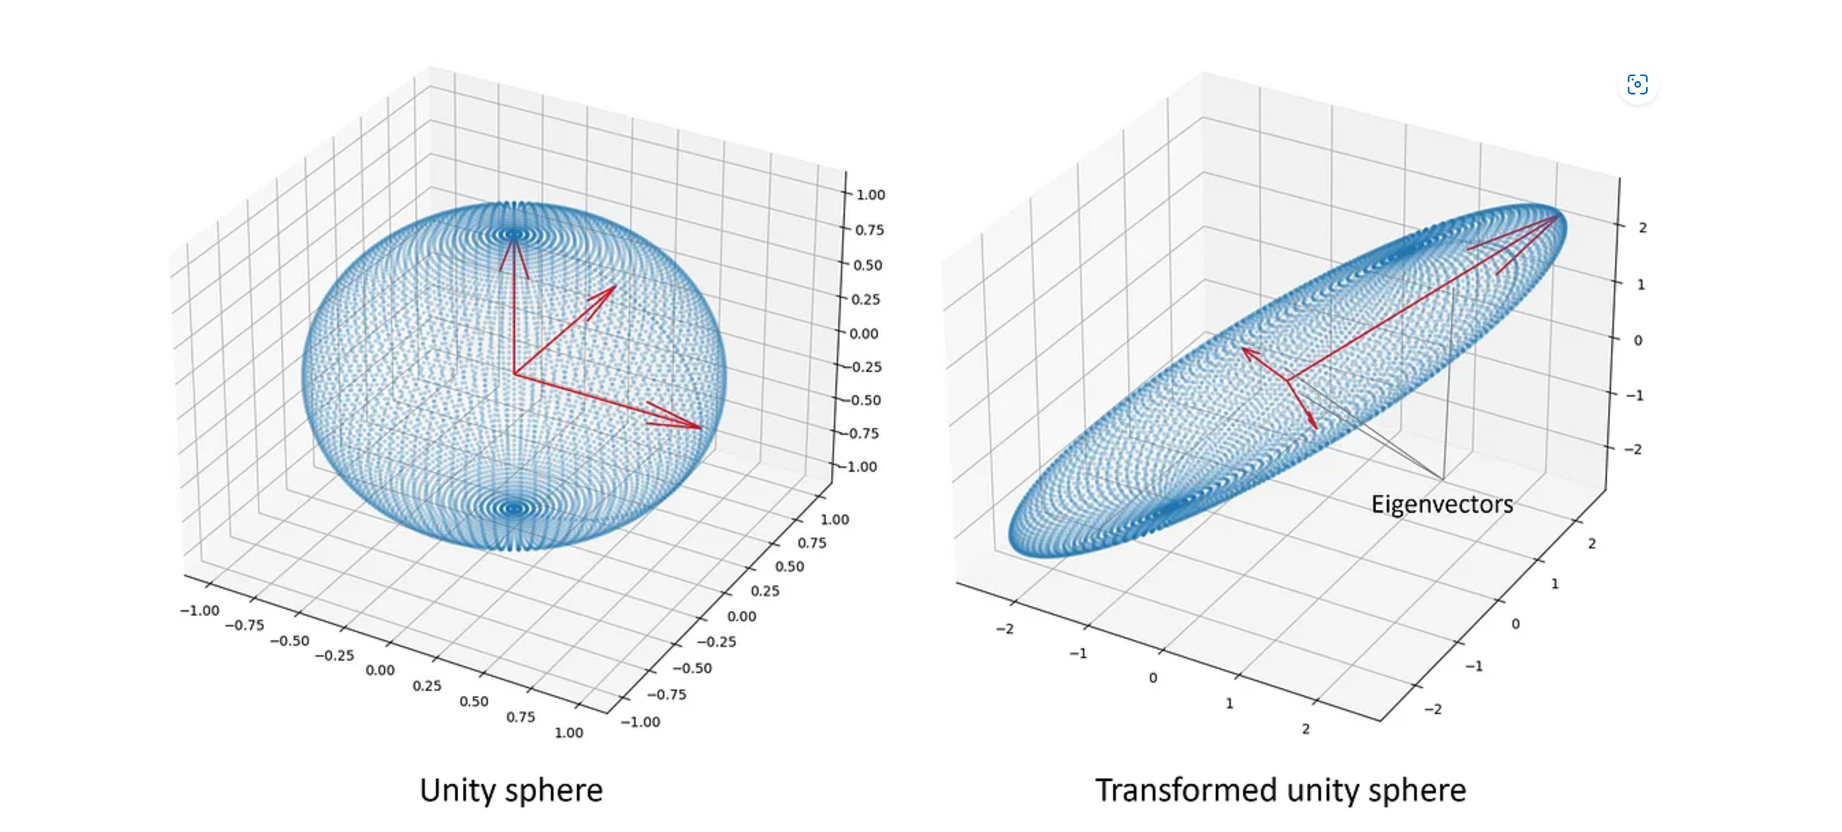
\includegraphics[width=0.8\textwidth]{C:/Users/marci/OneDrive/Pulpit/Opty - prezentacja/unity_transf_unity.png}
    
    \bigskip
    \textbf{Obrazek przedstawia:}
    \begin{itemize}
        \item Jak dane przekształcają się w przestrzeni, gdy używamy wektorów własnych.
        \item Wektory własne pokazują kierunki rozciągania danych, co pomaga w lepszej separacji klas.
    \end{itemize}
\end{frame}



\begin{frame}{Jak działają wektory własne?}
    W przestrzeni 3D możemy mieć więcej niż jeden wektor własny. W tym przypadku zazwyczaj wybieramy tylko te, które najlepiej rozdzielają klasy.

    \bigskip
    \textbf{Jak to działa w praktyce?}  
    \begin{itemize}
        \item W przestrzeni 3D mamy trzy główne wektory, które wskazują kierunki o największej zmienności danych.
        \item W LDA, dla dwóch klas, zazwyczaj wystarcza tylko jeden wektor, aby efektywnie oddzielić klasy.
        \item Dla większej liczby klas możemy wybrać więcej wektorów, ale w podstawowych przypadkach wystarczy jeden.
    \end{itemize}

    \bigskip
    \textbf{Obrazek przedstawia:}
    \begin{itemize}
        \item Jak dane przekształcają się w przestrzeni, gdy używamy wektorów własnych.
        \item Przekształcenie pozwala lepiej rozdzielić klasy.
    \end{itemize}

\end{frame}





% Slajd 4: Zrozumienie macierzy rozrzutu
\begin{frame}
    \frametitle{Macierz rozrzutu między klasami \( S_B \)}

    \begin{itemize}
        \item \textbf{Macierz rozrzutu między klasami \( S_B \):}  
        Mierzy, jak różnią się średnie poszczególnych klas w stosunku do globalnej średniej. Celem jest zmaksymalizowanie tej różnicy, aby klasy były jak najbardziej oddzielone.
    \end{itemize}

    \bigskip
    \textbf{Wzór na macierz rozrzutu między klasami:}
    \[
    S_B = \sum_{i=1}^{k} N_i (\mu_i - \mu)(\mu_i - \mu)^T
    \]
    Gdzie:
    \begin{itemize}
        \item \( N_i \) – liczba próbek w klasie \( i \),
        \item \( \mu_i \) – średnia klasy \( i \),
        \item \( \mu \) – globalna średnia wszystkich próbek.
    \end{itemize}
\end{frame}

\begin{frame}
    \frametitle{Macierz rozrzutu wewnątrz klas \( S_W \)}

    \begin{itemize}
        \item \textbf{Macierz rozrzutu wewnątrz klas \( S_W \):}  
        Mierzy, jak rozproszone są punkty danych w obrębie każdej klasy. Celem jest minimalizacja tej zmienności, aby dane w obrębie każdej klasy były jak najbardziej jednorodne.
    \end{itemize}

    \bigskip
    \textbf{Wzór na macierz rozrzutu wewnątrz klas:}
    \[
    S_W = \sum_{i=1}^{k} \sum_{x_j \in C_i} (x_j - \mu_i)(x_j - \mu_i)^T
    \]
    Gdzie:
    \begin{itemize}
        \item \( C_i \) – zbiór punktów należących do klasy \( i \),
        \item \( x_j \) – pojedyncza próbka w klasie \( i \),
        \item \( \mu_i \) – średnia klasy \( i \).
    \end{itemize}
\end{frame}



\begin{frame}
    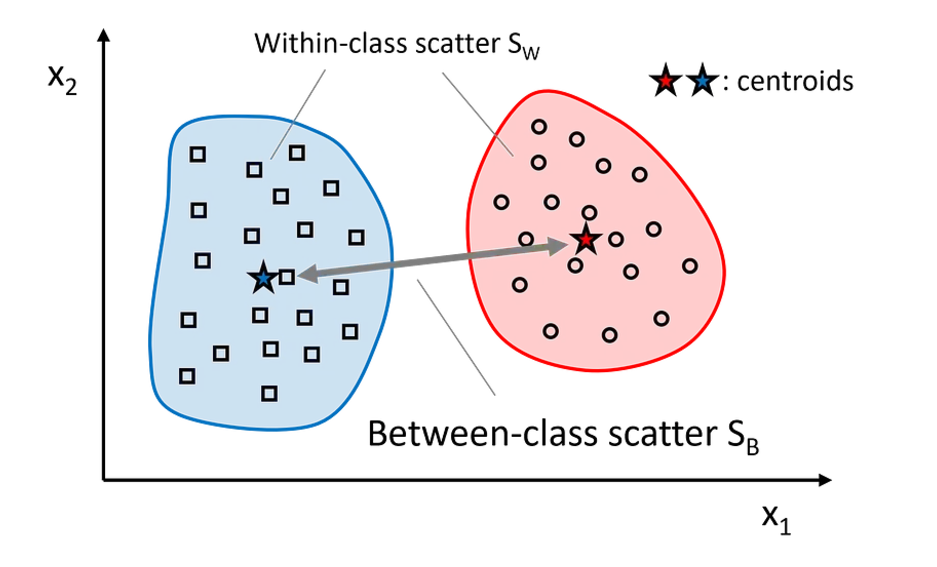
\includegraphics[width=0.8\textwidth]{C:/Users/marci/OneDrive/Pulpit/Opty - prezentacja/rys.png}
    
    \bigskip
    \begin{itemize}
        \item Intuicyjnie rozproszenie wewnątrz klasy sprawdza, jak zwarta jest każda klasa.
        \item Rozproszenie między klasami bada, jak daleko od siebie znajdują się różne klasy.
    \end{itemize}
\end{frame}



% Slajd 5: Rozróżnianie między klasami
\begin{frame}
    \frametitle{Rozróżnianie między klasami}
    Fisherowska dyskryminacja liniowa dąży do znalezienia najlepszego wektora \( \mathbf{w} \), który maksymalizuje rozróżnienie między klasami. Celem jest:
    \begin{itemize}
        \item Projektowanie przestrzeni, w której różnice między klasami są jak najbardziej widoczne.
        \item Projekcja danych na wektor \( \mathbf{w} \) pozwala na łatwiejsze przypisanie nowych danych do odpowiednich klas.
    \end{itemize}
\end{frame}



% Slajd 6: Przykład zastosowania w klasyfikacji roślin
\begin{frame}
    \frametitle{Przykład zastosowania}
    Załóżmy, że mamy dane dotyczące roślin i chcemy je sklasyfikować na podstawie cech takich jak długość i szerokość liści. 
    \begin{itemize}
        \item Wybieramy dwie cechy (np. długość i szerokość liści).
        \item Fisherowska dyskryminacja liniowa oblicza najlepszą linię separującą te dwie klasy.
    \end{itemize}
    
    Dzięki tej metodzie możemy łatwo oddzielić klasy roślin na podstawie dwóch prostych cech.
\end{frame}

% Slajd 7: Wykorzystanie LDA w analizie twarzy
\begin{frame}
    \frametitle{Zastosowanie w rozpoznawaniu twarzy}
    LDA jest także szeroko stosowane w rozpoznawaniu twarzy, gdzie cechy twarzy (np. odległości między oczami, szerokość nosa) służą do klasyfikacji osób.
    \begin{itemize}
        \item Twarze osób są reprezentowane jako wektory cech.
        \item LDA znajduje projekcję, która maksymalizuje różnice między twarzami różnych osób.
    \end{itemize}
    \textit{"Rozpoznawanie twarzy jest jednym z najczęściej stosowanych zastosowań LDA."}
\end{frame}

% Slajd 8: Zastosowanie w analizie tekstów
\begin{frame}
    \frametitle{Zastosowanie w analizie tekstów}
    LDA może być również wykorzystywana w analizie tekstów. Na przykład w klasyfikacji e-maili na spam i nie-spam:
    \begin{itemize}
        \item Cechy: obecność słów, długość e-maila, liczba załączników.
        \item LDA identyfikuje najlepsze cechy, które pozwalają na skuteczną klasyfikację.
    \end{itemize}
    \textit{„Fisherowska dyskryminacja liniowa jest bardzo efektywna w zadaniach klasyfikacji tekstów.”}
\end{frame}

% Slajd 9: Przykład z danymi medycznymi
\begin{frame}
    \frametitle{Przykład z danymi medycznymi}
    LDA jest także używane w medycynie, np. w klasyfikacji przypadków chorób:
    \begin{itemize}
        \item Zbieramy dane o pacjentach, np. wyniki badań krwi, ciśnienie.
        \item LDA pomaga oddzielić pacjentów zdrowych od chorych na podstawie cech medycznych.
    \end{itemize}
\end{frame}

% Slajd 10: Wzór na linię separującą
\begin{frame}
    \frametitle{Wzór na linię separującą}
    Jeśli mamy dane 2D, najlepsza linia separująca jest opisana przez wzór:
    \[
    \mathbf{w}^T \mathbf{x} + b = 0
    \]
    Gdzie:
    \begin{itemize}
        \item \( \mathbf{w} \) to wektor wag (prostopadły do linii),
        \item \( \mathbf{x} \) to dane (punkt na wykresie),
        \item \( b \) to przesunięcie (odległość od początku układu współrzędnych).
    \end{itemize}
\end{frame}

% Slajd 11: Wnioski
\begin{frame}
    \frametitle{Wnioski}
    Fisherowska dyskryminacja liniowa jest prostą, ale potężną techniką klasyfikacji. Znajduje szerokie zastosowanie w różnych dziedzinach, takich jak medycyna, analiza twarzy czy analiza tekstów. Choć jest to technika liniowa, może być wystarczająca w wielu praktycznych zastosowaniach.
\end{frame}

% Slajd 12: Bibliografia
\begin{frame}
    \frametitle{Bibliografia}
    \begin{itemize}
        \item Fisher, R. A. (1936). "The Use of Multiple Measurements in Taxonomic Problems". \textit{Annals of Eugenics}.
        \item Bishop, C. M. (2006). "Pattern Recognition and Machine Learning". \textit{Springer}.
        \item James, G., Witten, D., Hastie, T., \& Tibshirani, R. (2013). "An Introduction to Statistical Learning". \textit{Springer}.
    \end{itemize}
\end{frame}

\end{document}
